\documentclass[10pt,twocolumn]{article}
% Shared preamble for the Swedish Science Mafia workshop papers (compile with: tectonic main.tex)
\usepackage[letterpaper,margin=0.75in,columnsep=0.28in]{geometry}
\usepackage[T1]{fontenc}
\usepackage{newtxtext,newtxmath}
\usepackage{microtype}
\usepackage{booktabs,tabularx,multirow,array}
\usepackage{graphicx}
\usepackage{xcolor}
\usepackage{enumitem}
\setlist{nosep,leftmargin=1.2em}
\usepackage[font=small,labelfont=bf]{caption}
\usepackage{titlesec}
\titleformat{\section}{\normalfont\large\bfseries}{\thesection}{0.6em}{}
\titleformat{\subsection}{\normalfont\normalsize\bfseries}{\thesubsection}{0.6em}{}
\titlespacing*{\section}{0pt}{1.1ex plus .3ex}{0.6ex}
\titlespacing*{\subsection}{0pt}{0.9ex plus .2ex}{0.4ex}
\usepackage[hidelinks]{hyperref}
\usepackage{url}
\newcommand{\code}[1]{\texttt{\small #1}}
\newcommand{\workshopnote}{\footnotesize Workshop draft, written during and after the AI\,$\times$\,Science Hackathon (London, 3--4 October 2026). Every number is taken from the team repository at commit \texttt{554abdc} unless marked otherwise; see the evidence appendix.}
\makeatletter
\renewcommand{\@maketitle}{%
  \begin{center}{\LARGE\bfseries \@title \par}\vskip 0.8em
  {\normalsize \@author \par}\vskip 0.4em {\footnotesize \@date\par}\end{center}\vskip 0.6em}
\makeatother

\usepackage{amsmath}
\usepackage{xspace}
\renewcommand{\workshopnote}{\footnotesize Workshop draft, written after the AI\,$\times$\,Science Hackathon (London, 3--4 October 2026). Every number is from \texttt{experiments/tsp-construct-v1} (pre-registered protocol, run log, raw per-instance results) in the team repository.}
\newcommand{\TideGap}{8.83}
\newcommand{\TideSec}{376}
\newcommand{\TideN}{3}
\newcommand{\MctsGap}{11.25}
\newcommand{\MctsSec}{30}
\newcommand{\MctsN}{200}
\newcommand{\HifoGap}{11.55}
\newcommand{\HifoSec}{225}
\newcommand{\HifoN}{50}
\newcommand{\HifoGapH}{10.66}
\newcommand{\HifoSecH}{12}
\newcommand{\HifoNH}{200}
\newcommand{\HtwoSentence}{For each of MCTS-AHD, HiFo-Prompt, ReEvo, AEL and RefineEvo's file, at every size, an interface method has shorter tours (paired 95\% CI below zero) and no larger time per instance, so the pre-registered H2, which covers all six released files, fails only because of Clade-AHD's.}
\newcommand{\HfourSentence}{On fresh instances from our own seeds (1,000 / 1,000 / 200), 54 of 54 pre-registered paired comparisons keep their sign (six of them are exact ties between nearest neighbour and Clade-AHD's file).}
\newcommand{\NoCacheAbstract}{0.35--11.7\,s per instance, still faster than every rollout-based LLM heuristic}
\newcommand{\NoCacheHtwo}{Greedy + 2-opt + Or-opt's times use a per-instance cache of its plan. Without it the tours are identical and it takes 0.35 / 2.1 / 11.7\,s per instance, still faster than MCTS-AHD, HiFo-Prompt and TIDE. The dominance over MCTS-AHD, HiFo-Prompt and RefineEvo's file also holds through farthest insertion, which has no cache. ReEvo and AEL, however, are faster than any uncached method we ran that beats them, so for those two the dominance relies on the cache.}
\newcommand{\NoCacheRow}{0.35}
\newcommand{\NoCacheRowH}{2.1}
\newcommand{\NoCacheRowT}{11.7}


\title{Nothing to Construct: Textbook Heuristics Beat LLM-Designed\\Step-by-Step TSP Heuristics Inside Their Own Interface}
\author{Swedish Science Mafia\\{\small AI\,$\times$\,Science Hackathon, London}}
\date{\workshopnote}

\begin{document}
\twocolumn[{\maketitle\begin{abstract}
More than a dozen papers on LLM-based automatic heuristic design (AHD) report progress on one TSP
benchmark. An LLM writes \code{select\_next\_node}, and the tour is built by appending its answers;
the only hand-designed baseline on random instances is nearest neighbour. We re-evaluated the task
on MCTS-AHD's released 1,000-instance test sets in a pre-registered study. The function receives the
whole distance matrix at every call, so a function of its arguments alone can compute any tour and emit it one node at a time. The benchmark's ceiling is therefore the optimum. A short numpy function (about 100 lines) that emits a greedy-edge tour improved by 2-opt and Or-opt is 1.85\%, 2.44\% and 2.85\% above optimal at
50, 100 and 200 cities, below every published step-by-step LLM result (best: 4.76\%, 6.47\%, 8.88\%). With a per-instance cache it runs in 0.015--0.13\,s per instance, about 50--2,800$\times$ faster than the rollout-based LLM heuristics ; without the cache it takes \NoCacheAbstract. Farthest
insertion (1977), emitted the same way, is 5.53\%, 7.49\% and 9.03\%. It beats every LLM-designed result in the MCTS-AHD lineage (MCTS-AHD, CALM, MoH, Clade-AHD, PathWise), and also beats MCTS-AHD on 14 TSPLIB instances (8.70\% against 11.17\%). Re-running six released LLM-designed heuristics in the original evaluation
loop, five are Pareto-dominated by classical methods. The sixth, Clade-AHD's released file, builds
exactly the nearest-neighbour tour. Finally, MCTS-AHD's 200-city reference optimum, 10.659, is 0.46\% below the optimum of its own test set (10.708 by LKH; confirmed by exact solves on a sample), which overstates every 200-city gap that uses it.
\end{abstract}\vspace{1.2em}}]

\section{Introduction}
Since 2023, more than a dozen papers on LLM-based automatic heuristic design (AHD) have reported
progress on the same small benchmark: \emph{step-by-step construction} for the Euclidean TSP. Examples
include AEL~\cite{ael}, ReEvo~\cite{reevo}, EoH~\cite{eoh}, MCTS-AHD~\cite{mctsahd},
CALM~\cite{calm}, MoH~\cite{moh}, HiFo-Prompt~\cite{hifo}, Clade-AHD~\cite{clade},
PathWise~\cite{pathwise}, TIDE~\cite{tide} and SimpleEvol~\cite{simpleevol}. An LLM writes the body of
\begin{center}\code{select\_next\_node(current\_node, destination\_node, unvisited\_nodes, distance\_matrix)}\end{center}
and the evaluator builds a tour by appending the function's answer once per step. Scores are mean
gaps to an LKH reference on uniform random instances with 50, 100 and 200 cities. On random
instances the only hand-designed baseline these papers report is nearest neighbour, which is about
23--26\% above optimal. Against that baseline the reported progress looks large: from 22.6\% to
9.7\% at $n=50$ in MCTS-AHD's Table~1~\cite{mctsahd}, and to 4.76\% in TIDE~\cite{tide}.

Two facts about the benchmark are easy to miss.
\begin{itemize}
\item \textbf{Strong classical constructions exist and are cheap.} Farthest insertion
(Rosenkrantz, Stearns and Lewis, 1977~\cite{rosenkrantz}) is a one-pass construction. It is about
5.5\% above optimal at $n=50$ on this distribution~\cite{kool}. Greedy edge with 2-opt and Or-opt
local search (1958--1976) gets within a few percent. These are textbook results~\cite{johnson}.
\item \textbf{The interface hands the function the whole instance.} \code{distance\_matrix} is
passed in full at every call. A function can therefore compute any tour it likes and return that
tour's next node. The best recent heuristics already use this partially: MCTS-AHD's released
heuristic runs a nearest-neighbour rollout for every candidate, HiFo-Prompt's paper describes MST look-ahead, and
TIDE runs 2-opt to convergence inside each call. We found no paper that normalises compute against classical methods.
\end{itemize}

\paragraph{Contributions.}
\begin{itemize}
\item \textbf{A re-evaluation} of the benchmark on MCTS-AHD's released 1,000-instance test sets and on
fresh draws. It covers the published leaderboard (13 papers), six released LLM-designed heuristics
re-run through the original evaluation loop, and classical constructions implemented
\emph{inside} the interface as numpy functions whose output depends only on the call's arguments. The protocol was pre-registered.
\item \textbf{The interface's ceiling is the optimum, at negligible cost.} Emitting a tour that
greedy edge, 2-opt and Or-opt build from the matrix (about 100 lines of numpy) beats every published
step-by-step result at every size. Emitting an LKH tour reaches the reference itself.
\item \textbf{The MCTS-AHD lineage is below a 1977 baseline.} Farthest insertion, emitted the same
way, beats every LLM-designed result in MCTS-AHD's table and in CALM, MoH, Clade-AHD and PathWise.
\item \textbf{Released heuristics are Pareto-dominated} in tour length and time by classical
methods. Clade-AHD's released file is behaviourally nearest neighbour. HiFo-Prompt's runs the same deterministic rollout eight times, so seven of the eight are wasted.
\item \textbf{A reference error.} MCTS-AHD's $n=200$ optimum (10.659), which SimpleEvol also uses, is 0.46\% below the optimum of MCTS-AHD's own released test set (LKH, confirmed by exact solves on a sample).
\end{itemize}
These findings mirror a companion study on FunSearch's online bin-packing benchmark. There,
Sum-of-Squares~\cite{csirik}, a 2006 algorithm that we found no LLM-AHD paper comparing against, beats the
LLM-designed heuristics.

\section{Benchmark and methods}\label{sec:method}
\paragraph{Task and evaluation.} We copy MCTS-AHD's evaluation loop verbatim; it is identical to
ReEvo's. The tour starts and ends at node 0, and each call receives copies of the unvisited set and
of the full distance matrix. The test sets are MCTS-AHD's released \code{test\{50,100,200\}} (1,000
uniform instances each). They regenerate exactly from \code{np.random.seed(1234)} with its
generator, and we checked their SHA-256 against the released files. Fresh sets
(1,000/1,000/200 instances) come from our own seeds. The reference is LKH~\cite{lkh} through
elkai (RUNS$=3$, MAX\_TRIALS$=n$). On 42 distinct checked instances (16 at $n=50$, 26 at $n=200$), heavier settings up to MCTS-AHD's (RUNS$=10$, MAX\_TRIALS$=10{,}000$) gave identical tours, and an integer program proved five of them optimal. The gap is the ratio of mean tour length to
mean LKH length, minus one, as in MCTS-AHD's Table~1.

\paragraph{Released LLM-designed heuristics.} We re-run the code each project ships, pinned to a
commit:
\begin{itemize}
\item MCTS-AHD's ``leading heuristic'' (\code{gpt.py});
\item HiFo-Prompt's released TSP heuristic;
\item ReEvo's best heuristic and AEL's, both from ReEvo's test notebook;
\item the \code{gpt.py} files of RefineEvo and Clade-AHD.
\end{itemize}
The last two, and HiFo-Prompt's file, may not be those papers' best heuristics (HiFo-Prompt's paper describes an MST-look-ahead heuristic; its released file uses quadtree regions and rollouts), so we report them as ``released'' and do not attribute their numbers to the papers. TIDE,
SimpleEvol, MoH, CALM and PathWise did not release theirs, and we use their published numbers.

\paragraph{Classical methods inside the interface.} Each is a \code{select\_next\_node} written in numpy whose answer depends only on its four arguments:
\begin{itemize}
\item \textbf{NN}: nearest neighbour.
\item \textbf{FI-emit}: build the farthest-insertion tour of all nodes from \code{distance\_matrix},
oriented from the destination, and return the node after \code{current\_node}.
\item \textbf{GLS-emit}: the same, with a greedy-edge tour improved by 2-opt~\cite{croes} and
Or-opt~\cite{or} to a joint local optimum. A per-instance cache avoids recomputation and changes speed, not answers; we report uncached times too.
\item \textbf{LKH-emit}: the LKH tour, emitted the same way. This is the ceiling, and it needs a
compiled solver.
\end{itemize}
FI-emit reproduces a standalone farthest-insertion implementation to within $10^{-14}$ on every development instance. A tempting alternative is to \emph{replan} farthest insertion from the current
node at every step. It is much worse (8.4\% against 5.7\% on development data), because anchoring
the residual path at the current node destroys farthest insertion's global skeleton. Planning once
from the full matrix is what makes the textbook algorithm expressible in this interface.

\paragraph{Pre-registration.} Before any heuristic touched a test set, we fixed the hypotheses, the
instance prefixes for the slow heuristics, and the statistics: paired per-instance differences with
95\% percentile bootstrap CIs (10,000 resamples) and win/tie/loss counts. A first draft hypothesised
only that farthest insertion beats every published result. The literature search showed three
rollout-based methods below it, so the hypotheses were revised before the run; both versions are in
the repository.

\section{Results}\label{sec:results}
\paragraph{Positive controls.} Our nearest neighbour reproduces MCTS-AHD's published
``Greedy Construct'' objectives on all three test sets: 6.959, 9.706 and 13.461. Our LKH means
reproduce its published optima at $n=50$ and 100 (5.6755 and 7.7680). At $n=200$ they do not
(10.708 against 10.659), which we examine at the end of this section. All gaps below are against our
reference.

\begin{table*}[t]\centering\small
\caption{Gap to the optimum (\%) and median wall seconds per instance on MCTS-AHD's released test sets
(1,000 instances each unless the count is given). \emph{Emitted}: a \code{select\_next\_node} that builds one tour from the distance matrix (a function of its arguments) and returns its next node; greedy and LKH cache the plan per instance, and the uncached row gives the cost without it.
Published rows are as printed. Times come from one shared, loaded laptop; read them as orders of
magnitude.}\label{tab:main}
\begin{tabular}{@{}llrrrrrr@{}}\toprule
& & \multicolumn{2}{c}{$n=50$} & \multicolumn{2}{c}{$n=100$} & \multicolumn{2}{c}{$n=200$}\\
\cmidrule(lr){3-4}\cmidrule(lr){5-6}\cmidrule(l){7-8}
Method & kind & gap & s & gap & s & gap & s\\\midrule
LKH, emitted (ceiling) & classical & 0.00 & 0.015 & 0.00 & 0.056 & 0.00 & 0.27\\
\textbf{Greedy edge + 2-opt + Or-opt, emitted} & classical & \textbf{1.85} & 0.015 & \textbf{2.44} & 0.045 & \textbf{2.85} & 0.13\\
\quad same, without the cache & classical & 1.85 & \NoCacheRow & 2.44 & \NoCacheRowH & 2.85 & \NoCacheRowT\\
Farthest insertion (1977), emitted & classical & 5.53 & 0.046 & 7.49 & 0.24 & 9.03 & 1.0\\
Nearest neighbour & classical & 22.62 & 0.0004 & 24.94 & 0.001 & 25.71 & 0.006\\\midrule
TIDE, appendix heuristic (transcribed) & LLM, re-run & 3.02 & 3.3 & 6.21 & 46 & \TideGap & \TideSec\\
& & \footnotesize(200 inst.) & & \footnotesize(30 inst.) & & \footnotesize(\TideN\ inst.) &\\
MCTS-AHD, released & LLM, re-run & 8.78 & 0.72 & 10.30 & 3.5 & \MctsGap & \MctsSec\\
& & & & & & \footnotesize(\MctsN\ inst.) &\\
HiFo-Prompt, released & LLM, re-run & 9.09 & 4.4 & \HifoGapH & \HifoSecH & \HifoGap & \HifoSec\\
& & & & \footnotesize(\HifoNH\ inst.) & & \footnotesize(\HifoN\ inst.) &\\
ReEvo, released & LLM, re-run & 10.46 & 0.021 & 11.87 & 0.15 & 13.01 & 0.96\\
AEL, released & LLM, re-run & 10.30 & 0.036 & 12.26 & 0.15 & 14.07 & 0.94\\
RefineEvo, released file & LLM, re-run & 11.71 & 0.071 & 12.65 & 0.34 & 13.76 & 1.9\\
Clade-AHD, released file & LLM, re-run & 22.62 & 0.001 & 24.94 & 0.004 & 25.71 & 0.015\\\midrule
TIDE~\cite{tide} & published & 4.76 & -- & 7.15 & -- & 10.65 & --\\
SimpleEvol~\cite{simpleevol} & published & 4.77 & -- & 6.47 & -- & 9.49 & --\\
HiFo-Prompt~\cite{hifo} & published & 6.63 & -- & 8.58 & -- & 8.88 & --\\
PathWise~\cite{pathwise} & published & 8.41 & -- & 11.85 & -- & 12.14 & --\\
MCTS-AHD~\cite{mctsahd} (GPT-4o-mini) & published & 9.69 & -- & 11.79 & -- & 13.71$^\dagger$ & --\\
MoH~\cite{moh} & published & 9.89 & -- & 11.44 & -- & 13.31 & --\\
CALM~\cite{calm} & published & 10.04 & -- & 11.58 & -- & 13.41 & --\\
Clade-AHD~\cite{clade} & published & 10.39 & -- & 9.22 & -- & 11.30 & --\\\bottomrule
\multicolumn{8}{@{}l}{\footnotesize $^\dagger$13.19 against the corrected optimum. Published rows use each paper's own test sets and references; see the repository's literature notes.}
\end{tabular}\end{table*}

\begin{figure*}[t]\centering
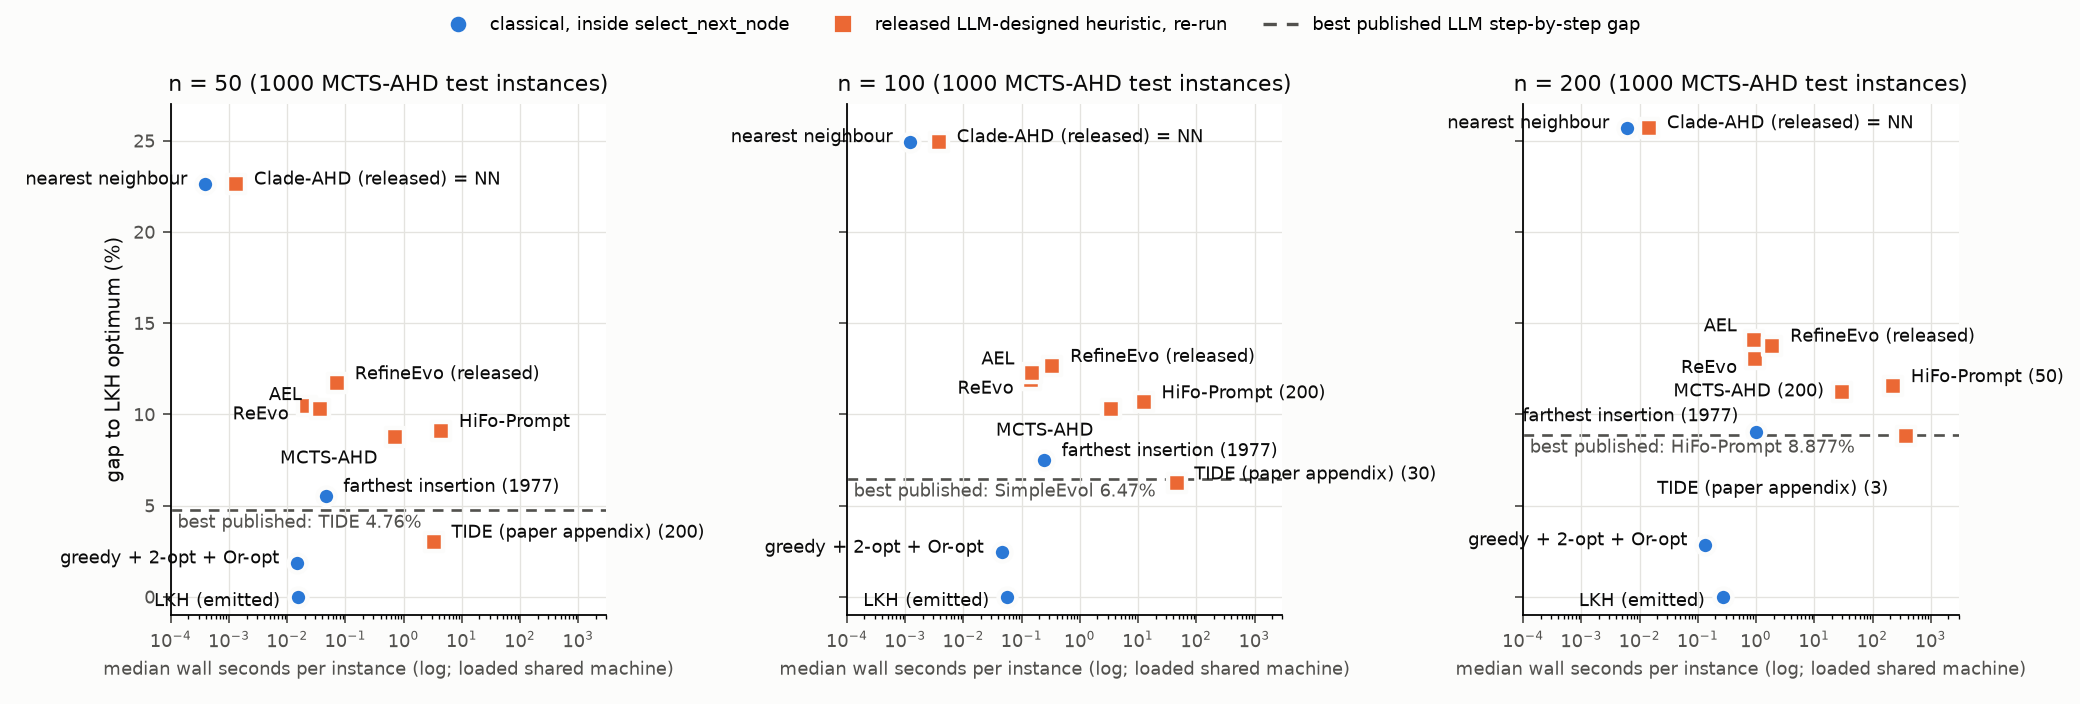
\includegraphics[width=\textwidth]{fig_pareto.png}
\caption{Gap against time per instance on MCTS-AHD's test sets. Blue: classical methods inside
\code{select\_next\_node}. Orange: released LLM-designed heuristics, re-run on the same instances and
machine. Dashed: best published step-by-step result. Classical methods occupy the whole lower-left
frontier.}\label{fig:pareto}
\end{figure*}

\paragraph{The interface's ceiling (H1).} Table~\ref{tab:main} and Figure~\ref{fig:pareto} show the
main result. Emitting a greedy-edge tour improved by 2-opt and Or-opt beats every published step-by-step result at every size (RedAHD, which drops the per-step interface, reports 1.62\% at $n=50$): 1.85\% against TIDE's 4.76\%, 2.44\% against SimpleEvol's
6.47\%, and 2.85\% against HiFo-Prompt's 8.88\%. It also beats RefineEvo's Claude Opus heuristic,
whose published objectives imply about 3.3\% and 4.7\% at $n=100$ and 200, and TIDE's own heuristic
re-run on the same instances. An emitted LKH tour reaches the reference. The benchmark therefore
does not bound what a \code{select\_next\_node} can achieve. It only bounds what the LLM search
chose to write.

\paragraph{A 1977 baseline (H3).} Farthest insertion, a one-pass construction with no local search and no cache, beats every LLM-AHD row of MCTS-AHD's Table~1 and of CALM, MoH, Clade-AHD and PathWise at every size (those tables also list POMO, a trained neural solver, which is not part of the comparison).
Against the released MCTS-AHD heuristic re-run on the same 1,000 instances at $n=50$, it is shorter
by 0.184 per instance (95\% CI $[-0.202,-0.167]$; 735 wins, 265 losses), and its CIs against
MCTS-AHD, ReEvo and AEL are below zero at every size. On MCTS-AHD's own TSPLIB protocol (the 14
instances in its repository), farthest insertion averages 8.70\% against MCTS-AHD's 11.17\% and
Christofides' 11.21\%. Greedy + 2-opt + Or-opt averages 2.38\% there. Even nearest neighbour with plain 2-opt (5.88 / 6.94 / 7.75\%) beats every LLM-AHD row of the MCTS-AHD lineage.

\paragraph{Released heuristics are Pareto-dominated (H2).} \HtwoSentence\ The exception is
Clade-AHD's released \code{gpt.py}. Its score is $0.5d - 1/(d+10^{-5})$ plus a constant, where $d$ is
the distance from the current node; this is increasing in $d$, so it always picks the nearest node,
and it reproduces nearest neighbour's tour on every instance. Nothing can be strictly faster and
better than it. HiFo-Prompt's released heuristic averages eight ``lookahead simulations'' that are
the same deterministic rollout; one gives identical tours, 6.9$\times$ faster. \NoCacheHtwo\ To give the LLMs their due, MCTS-AHD's blend (0.7 immediate distance, 0.3 rollout, plus a centre penalty) beats a textbook
nearest-neighbour rollout (8.78\% against 10.82\%).

\paragraph{Robustness (H4).} \HfourSentence

\paragraph{The $n=200$ reference.} MCTS-AHD's Table~1 lists 10.659 as the optimal mean at $n=200$.
On its released test200, the instances that reproduce its nearest-neighbour objective exactly, our LKH mean is 10.708, and the evidence says it is the optimum:
\begin{itemize}
\item our LKH setting matched MCTS-AHD's heavier LKH setting on 20 of 20 instances;
\item an integer program (HiGHS with subtour cuts) proved our tours optimal on 5 of 5 instances;
\item PathWise independently reports 10.709 on its own 250 instances.
\end{itemize}
Gaps computed against 10.659 are therefore overstated by about 0.5 points: MCTS-AHD's 13.71\% is
13.19\%. SimpleEvol and CALM print the same 10.659 as their reference, and Clade-AHD's $n=200$ numbers imply it. At $n=50$ and 100 the published
references are correct.

\section{Related work}\label{sec:related}
\paragraph{Classical tour construction.} Insertion heuristics were analysed by Rosenkrantz, Stearns
and Lewis~\cite{rosenkrantz}. Their empirical behaviour on random uniform instances is catalogued by
Johnson and McGeoch~\cite{johnson} and the DIMACS TSP Challenge. Farthest insertion is the
strongest of the simple insertion rules. Savings~\cite{clarke} and Christofides are stronger at
large $n$. 2-opt~\cite{croes} and Or-opt~\cite{or} remove most of the remaining excess.
Rollout~\cite{bertsekas} is the classical way to turn a construction into a look-ahead policy, and
it is what several LLM-designed heuristics rediscover.

\paragraph{Neural and LLM-based heuristic design.} Kool et al.~\cite{kool} report insertion
heuristics next to learned constructive policies on exactly this distribution. We found no LLM-AHD paper that keeps that practice on the standard random test sets. Among the papers we found, only RouteRepair~\cite{routerepair}
places farthest insertion next to an LLM constructor: with its own adapter, its LLM construction is 9--11 points worse at $n=50$--$200$. It does not relate this to the MCTS-AHD leaderboard. RedAHD~\cite{redahd}
drops the per-step interface and writes whole-route functions with 2-opt. The critiques of LLM-AHD benchmarks we found target bin packing~\cite{herrmann,sim}, or called for stronger
\emph{search} baselines~\cite{zhang}, not classical algorithms. MOSAIC~\cite{mosaic} notes that
single-pass scoring prompts exclude look-ahead, and responds by permitting it.

\section{Discussion}\label{sec:discussion}
\paragraph{What the leaderboard measures.} With the whole matrix in every call, the step-by-step
interface constrains the \emph{output format}, not the algorithm. Any tour can be emitted, so the
ceiling is the optimum, and a short numpy function gets within a few percent of it. A published gap
on this benchmark therefore mixes two things: what the LLM search found, and how much computation
the found function is allowed per call. Recent gains come from the second. TIDE's heuristic runs
2-opt to convergence for up to 12 candidates at every step; HiFo-Prompt's runs a full
nearest-neighbour rollout per candidate, eight times. Without a compute budget, these numbers cannot
be compared with each other or with one-pass constructions.

\paragraph{Recommendations for this benchmark.}
\begin{enumerate}
\item \textbf{Report the classical baselines that fit the interface.} At minimum farthest
insertion, and a construction with 2-opt/Or-opt as the emitted reference.
\item \textbf{Report time per instance against those baselines on the same machine,} or fix a budget
per call.
\item \textbf{If the intent is to study one-pass construction rules, enforce it.} For example, pass
only the current node's row and the destination's row, or count matrix accesses.
\item \textbf{Publish per-instance reference values} with the test sets.
\end{enumerate}

\paragraph{Scope.} We study one benchmark task in one interface, on uniform instances up to 200
cities. We make no claim about LLM-AHD in general, or about frameworks in which the LLM designs
components of strong solvers (GLS, ACO, LKH parameters). Those tasks report strong solver baselines
already. Our timings come from a shared, loaded laptop; only orders of magnitude should be read
from them. Our point is narrower and, we think, actionable: on this widely used task, progress claims on random instances have been made against nearest neighbour, while textbook methods expressible inside the same interface were absent from the standard evaluation.


\begin{thebibliography}{99}
\setlength{\itemsep}{1pt}\small
\bibitem{ael} F. Liu, X. Tong, M. Yuan and Q. Zhang. Algorithm evolution using large language model. arXiv:2311.15249, 2023.
\bibitem{eoh} F. Liu et al. Evolution of heuristics: towards efficient automatic algorithm design using large language model. \emph{ICML}, 2024. arXiv:2401.02051.
\bibitem{reevo} H. Ye et al. ReEvo: large language models as hyper-heuristics with reflective evolution. \emph{NeurIPS}, 2024. arXiv:2402.01145.
\bibitem{mctsahd} Z. Zheng, Z. Xie, Z. Wang and B. Hooi. Monte Carlo tree search for comprehensive exploration in LLM-based automatic heuristic design. \emph{ICML}, 2025. arXiv:2501.08603.
\bibitem{calm} CALM. arXiv:2505.12285, 2025.
\bibitem{moh} MoH. arXiv:2505.20881, 2025.
\bibitem{hifo} HiFo-Prompt: prompting with hindsight and foresight for LLM-based automatic heuristic design. arXiv:2508.13333, 2025.
\bibitem{clade} Beyond the node: clade-level selection for efficient MCTS in automatic heuristic design. arXiv:2602.00549, 2026.
\bibitem{pathwise} PathWise. arXiv:2601.20539, 2026.
\bibitem{tide} C. Chen, M. Zhong, Y. Fan, J. Shi and J. Sun. TIDE: tuning-integrated dynamic evolution for LLM-based automated heuristic design. arXiv:2601.21239, 2026.
\bibitem{simpleevol} SimpleEvol. arXiv:2609.37172, 2026.
\bibitem{refineevo} RefineEvo. arXiv:2607.11358, 2026.
\bibitem{routerepair} RouteRepair. arXiv:2609.11452, 2026.
\bibitem{redahd} RedAHD. arXiv:2505.20242, 2025.
\bibitem{mosaic} MOSAIC. arXiv:2608.07544, 2026.
\bibitem{zhang} R. Zhang et al. Understanding the importance of evolutionary search in automated heuristic design with large language models. \emph{PPSN}, 2024. arXiv:2407.10873.
\bibitem{herrmann} J. Herrmann and G. Pallez. An in-depth study of LLM contributions to the bin packing problem. arXiv:2510.27353, 2025.
\bibitem{sim} Sim, Renau and Hart. Beyond the hype: benchmarking LLM-evolved heuristics for bin packing. \emph{EvoApplications}, 2025. arXiv:2501.11411.
\bibitem{kool} W. Kool, H. van Hoof and M. Welling. Attention, learn to solve routing problems! \emph{ICLR}, 2019. arXiv:1803.08475.
\bibitem{rosenkrantz} D. J. Rosenkrantz, R. E. Stearns and P. M. Lewis. An analysis of several heuristics for the traveling salesman problem. \emph{SIAM J. Comput.} 6(3):563--581, 1977.
\bibitem{croes} G. A. Croes. A method for solving traveling-salesman problems. \emph{Operations Research} 6(6):791--812, 1958.
\bibitem{or} I. Or. Traveling salesman-type combinatorial problems and their relation to the logistics of regional blood banking. PhD thesis, Northwestern University, 1976.
\bibitem{clarke} G. Clarke and J. W. Wright. Scheduling of vehicles from a central depot to a number of delivery points. \emph{Operations Research} 12(4):568--581, 1964.
\bibitem{johnson} D. S. Johnson and L. A. McGeoch. The traveling salesman problem: a case study in local optimization. In \emph{Local Search in Combinatorial Optimization}, Wiley, 1997.
\bibitem{lkh} K. Helsgaun. An effective implementation of the Lin--Kernighan traveling salesman heuristic. \emph{EJOR} 126(1):106--130, 2000.
\bibitem{bertsekas} D. P. Bertsekas, J. N. Tsitsiklis and C. Wu. Rollout algorithms for combinatorial optimization. \emph{J. Heuristics} 3:245--262, 1997.
\bibitem{csirik} J. Csirik et al. On the sum-of-squares algorithm for bin packing. \emph{J. ACM} 53(1):1--65, 2006.
\end{thebibliography}
\end{document}
